\chapter{Ergebnisse}
\thispagestyle{fancy}
\section{Untersuchung optisch gepumpter Laserstrukturen auf unterschiedlichen Templates}




Dieses Kapitel widmet sich der Untersuchung der zweier Probenreihen der Serie 1 und Serie 2 von optisch gepumpten Laserstrukturen, die aus Rezepten aus zwei unterschiedlichen Serien stammen. Die beiden Serien unterscheiden sich im wesentlichen dadurch, dass sie mit(Serie 2) und ohne Übergitter(Serie 1) gewachsen wurden. Jede Reihe für sich weist  zusätzlich noch Unterschiede in den Proben auf, so sind zwei Proben der Reihe Serie 1 auf AlN-Bulk zweier unterschiedlicher Hersteller (HexaTech, IKZ) gewachsen und alle anderen Proben auf ELO AlN/Sapphire mit jeweils 3 unterschiedlichen "Offcut"-Winkeln. Tabellarisch sieht die Zusammenstellung wie folgt aus: 

\vspace{1cm}


\setlength{\arrayrulewidth}{0.1mm}
\setlength{\tabcolsep}{4.5mm}
\renewcommand{\arraystretch}{1.5}
 
\centering
\begin{tabular}{ |c|c|c|c|c|c|   }
\hline
\multicolumn{3}{|c|}{Serie 1} & \multicolumn{3}{c|}{Serie 2}  \\
\hline
Endung & offcut& Template & Endung & offcut & Template \\
\hline
A & 0.1$^\circ$m & Bulk(IKZ) &A & 0.2$^\circ$m & ELO \\
B & 0.1$^\circ$m & ELO & B & 0.1$^\circ$m & ELO \\
C & 0.1$^\circ$m* & ELO & C & 0.1$^\circ$m* & ELO \\
D & 0.2$^\circ$m & ELO &  & &  \\
E & 0.1$^\circ$m & Bulk(Hexatech) & & & \\
\hline
\end{tabular}
\newpage




\begin{figure}[htb]
    \centering
    \begin{minipage}[t]{0.49\linewidth}
        \centering
        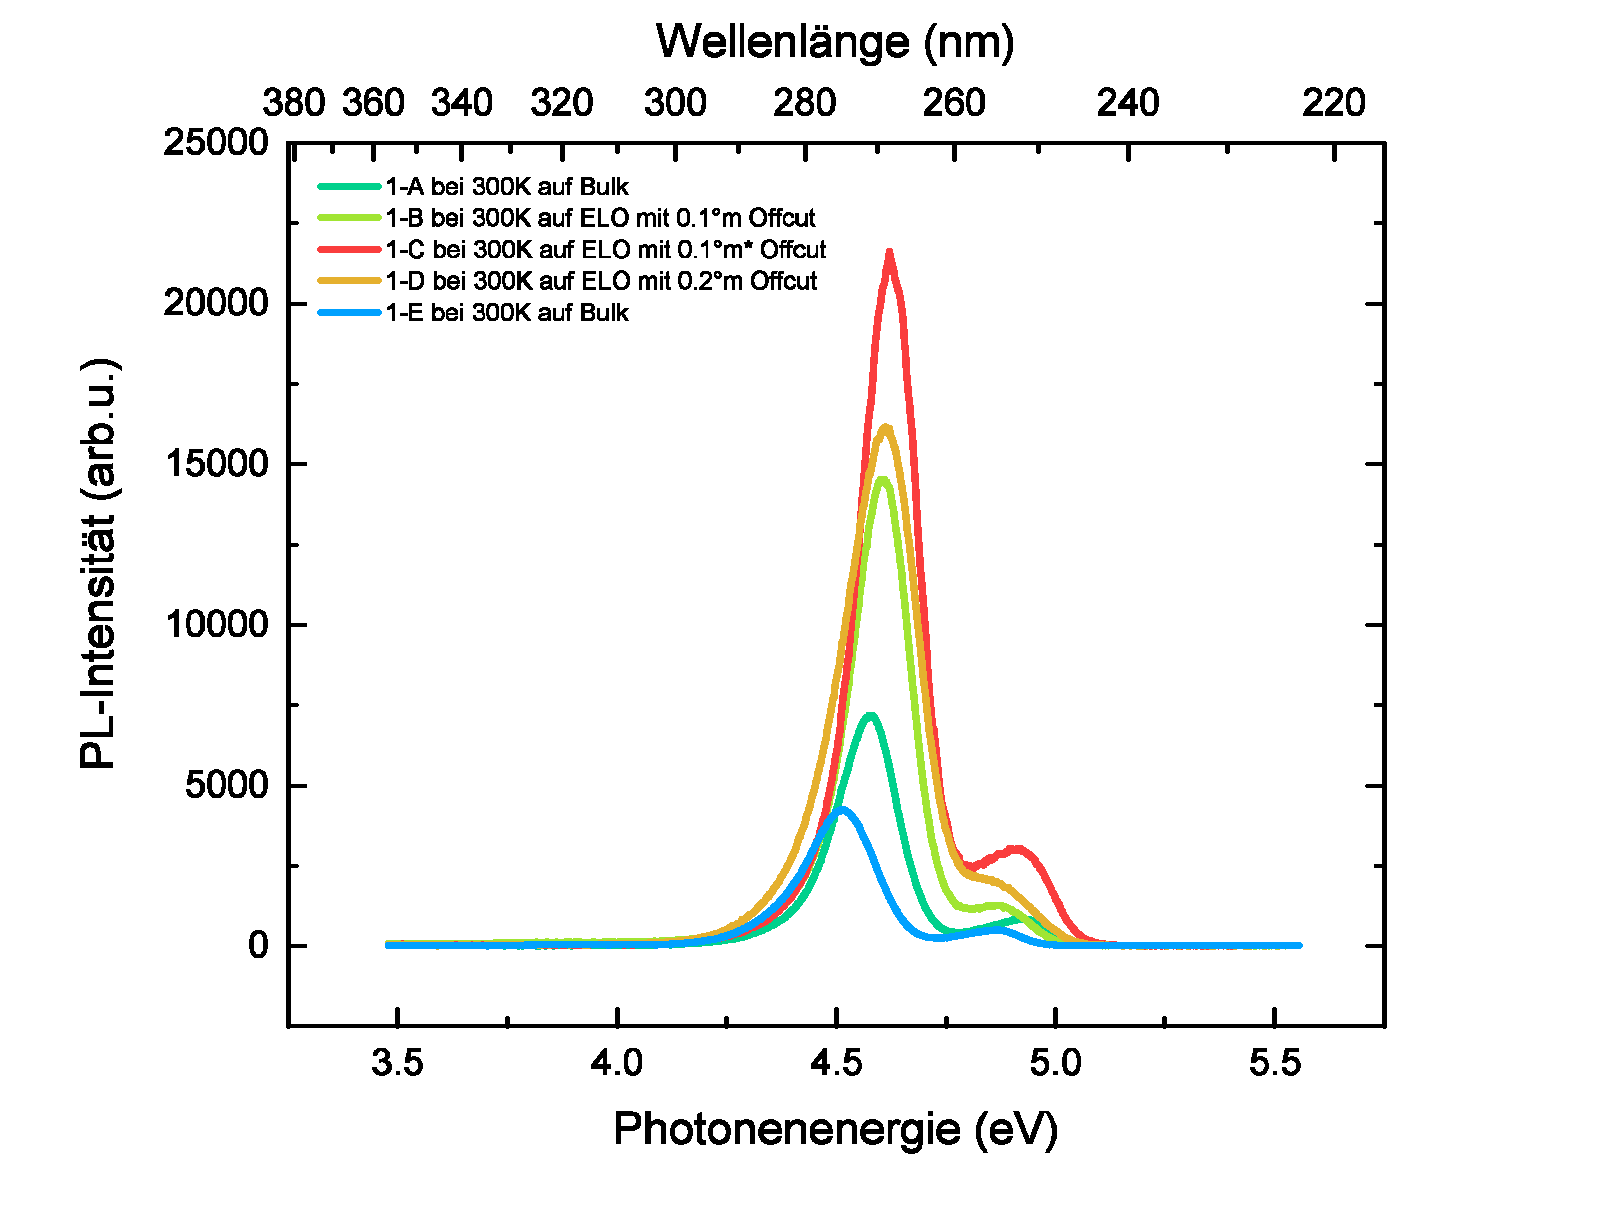
\includegraphics[width=\linewidth]{Bilder/TS4045Uebersicht.pdf}
        \caption{PL-Spektren der Proben ohne Übergitter}
    \end{minipage}% <- sonst wird hier ein Leerzeichen eingefügt
    \hfill
    \begin{minipage}[t]{0.49\linewidth}
        \centering
        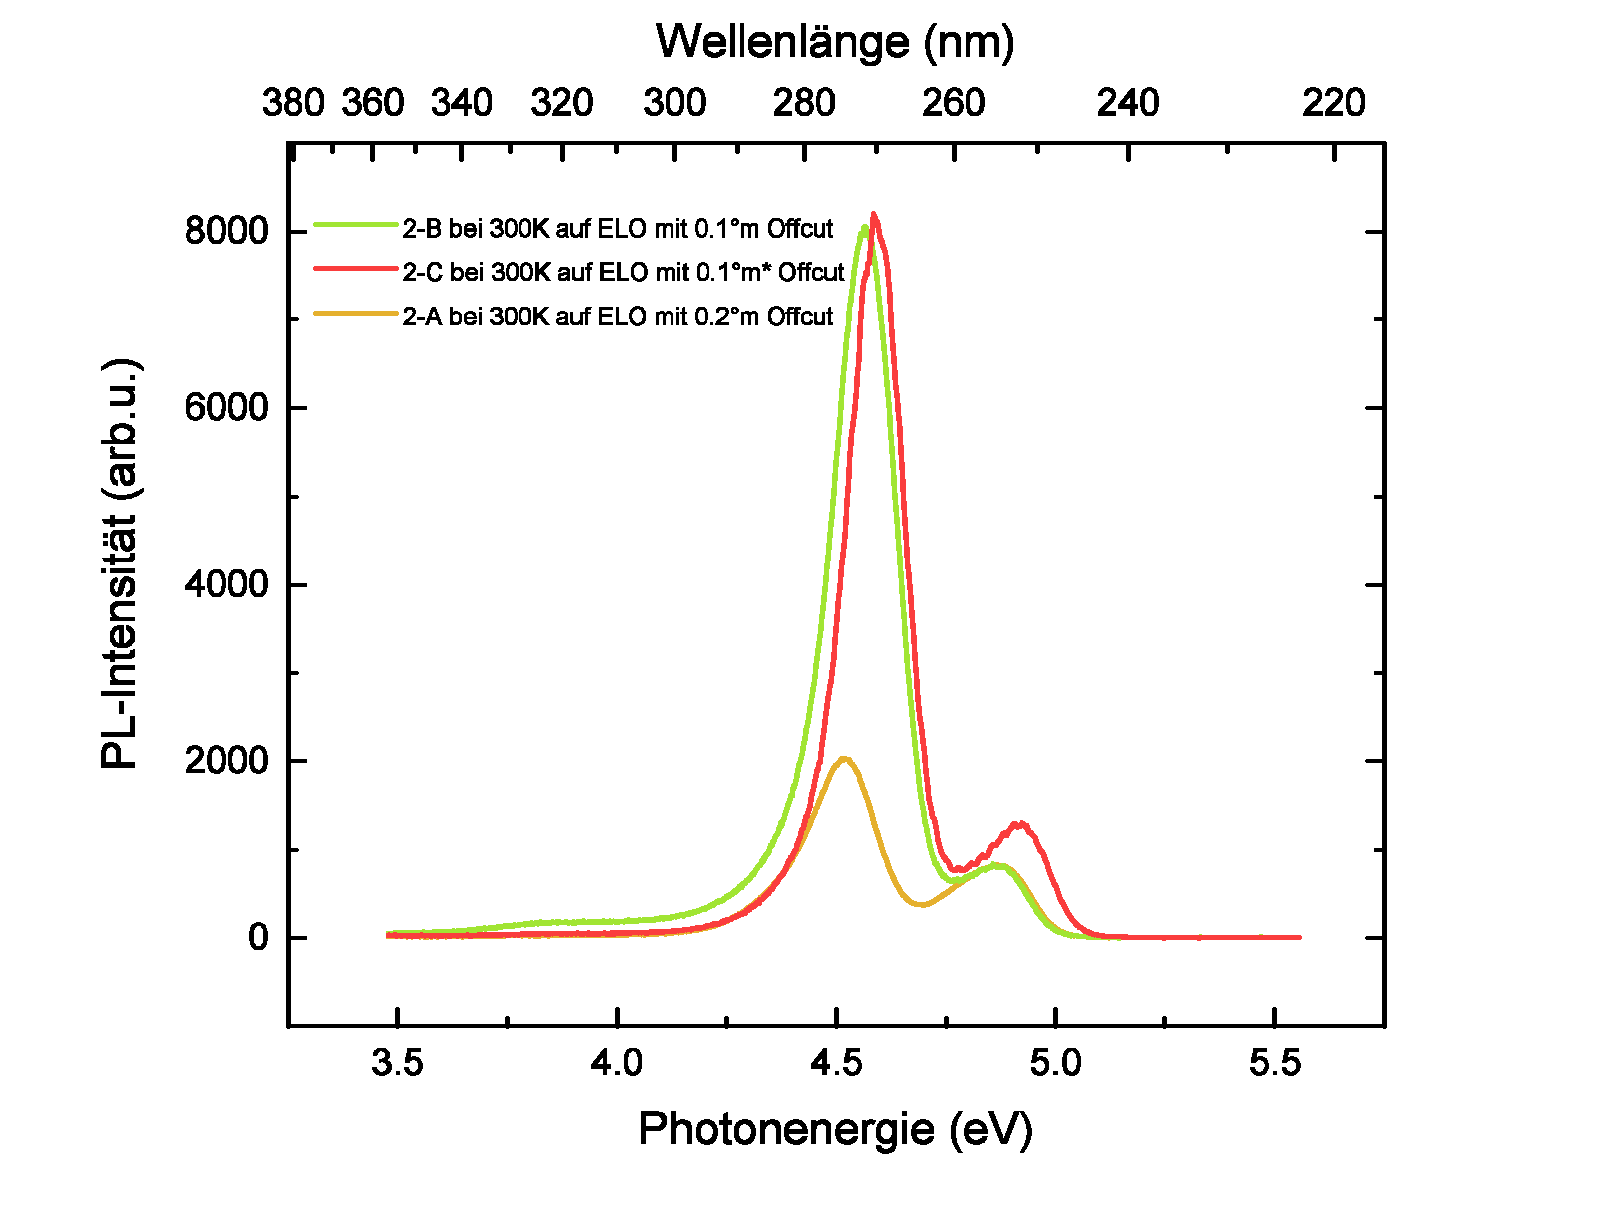
\includegraphics[width=\linewidth]{Bilder/TS4048Uebersicht.pdf}
        \caption{PL-Spektren der Proben mit Übergitter}
    \end{minipage}
\end{figure}






